%%%%%%%%%%%%%%%%%%%%%%%%%%%%%%%%%%%%%%%%%%%%
\subsection{Work-flow overview}

The ultimate goal of the PFS commissioning work-flow is to optimize the PFS performance and validate the goodness for scientific use.
To achieve this goal, we proceed the PFS commissioning following this outline:
\begin{enumerate}
\item Integrate PFS subsystems of which the performances have been validated by the PFS collaborators.
\item Operate the system and confirm their functions on the telescope.
\item Characterize the system, e.g. by calibrating the coordinate systems to put the fibers on the targets with required accuracy.
\item Evaluate the on-sky performance and validate it. \\
Firstly we focus on verifying the performances at given telescope positions, rotation angles even if we cannot confirm the same performance at all positions.
\item Finally, stabilize the instrument performances. \\
We optimize software, re-configuration sequence, calibration and so on.
We validate the performance at any telescope pointing or time.
\end{enumerate}

The latest top-level requirements are described on the following page: \\
{\tt http://sumire.pbworks.com/w/page/76118150/System\%20level\%20requirements}\\
See also the compliance matrix in section \ref{sec:cmatrix}.

\bigskip

The work-flow of the PFS commissioning (Fig. \ref{fig:flowchart}) consists of five parts: 
\begin{enumerate}
\item Validation of MCS (labeled with M-\#, see section \ref{sec:MCS})
 \begin{itemize}
 \item Validation of MCS basic functions.
 \item Pre-study of the coordinate transformation using pinhole array on POpt2.
 \end{itemize}
This part requires only MCS.
\item Validation of PFI (labeled with P-\#, see section \ref{sec:PFI}), basically prior to SpS delivery at Subaru.
 \begin{itemize}
 \item Alignment of WFC with the primary mirror.
 \item Telescope pointing analysis.
 \item AG camera validation.
 \item Confirmation of PFI--MCS relation (registration of Fixed Fiducial Fibers in F3C).
 \item Make the first-pass distortion map using AGCs (sky).
 \end{itemize}
This part requires only PFI basically, but some processes need MCS, too.
\item Validation of SpS (labeled with S-\#, see section \ref{sec:SpS})
 \begin{itemize}
 \item Validation of image quality and stability in the SCR.
 \item Characterization of SMs.
 \end{itemize}
This part requires SMs and SCR.
We don't need the telescope to carry out this part.
\item Validation of FoCCoS--Cable B (labeled with F-\#, see section \ref{sec:FoCCoS})
 \begin{itemize}
 \item Validation of cable connection.
 \item Confirmation of fibers ID on MCS and SpS.
 \end{itemize}
This part requires all subsystems: MCS, PFI, Cable B and SpS.
\item Commissioning of all systems (labeled with A-\#, see section \ref{sec:All}
 \begin{itemize}
 \item Cobra calibration.
 \item PSF characterization.
 \item Make the second-pass distortion map using fibers (sky).
 \item Validation of all observational sequence.
 \item Fiber-reconfiguration.
 \item Performance verification:
 	\begin{itemize}
	\item Flux calibration
	\item Sky subtraction
	\item Total throughput
	\item Maximum exposure time of one frame, and stacking for long time ($>$ 10 hours) exposure
	\item Quality Assurance procedure
	\item Beam-switching mode
 \end{itemize}
 \item Stabilization of the instrument performance and operation.
 \end{itemize}
This part requires all subsystems: MCS, PFI, Cable B and SpS.
\end{enumerate}

During the commissioning procedure, we also verify the software sequence for observation (acquisition, fiber configuration, guiding, and exposure) at suitable commissioning sequences.
We also verify the data reduction pipeline (DRP), and quality-assurance (QA) process and so on.


%---------------------------------------------------
% Figure: Big picture of the PFS commissioning
%---------------------------------------------------
\begin{landscape}
\begin{figure}[!ht]
\begin{center}
\vspace*{80mm}
\hspace*{-10mm}
\includegraphics[width=235mm]{PFScommissioning.pdf}
\end{center}
\vspace*{-90mm}
\caption{Flowchart of Validation \& Commissioning. Larger one is available on the PBworks: \newline
http://sumire.pbworks.com/w/file/101350174/PFScommissioning.pdf
%http://member.ipmu.jp/yuki.moritani/tmp/PFS/PFScommissioning.pdf
}
\label{fig:flowchart}
\end{figure}
\end{landscape}

%%% Subsystem I \& T and capable functions at delivery
\subsection{Subsystem I \& T (TBD)}
\subsubsection{I \& T at Subaru}
Each subsystem is delivered to Subaru separately.
After the delivery, collaborators will re-assemble modules (if needed) and test their performance.
In this section, the brief summary of I\&T of subsystems are described.
See the documents by collaborators (TBA) for detailed procedure of I\&T.

Table \ref{tbl:SubSysIandT} summarizes schedule and place of I\&T of subsystems.
The validated functions before shipping (or before commissioning) is listed in Table \ref{tbl:subfuncs}.
The file named {\tt PFS\_AIT\_Subaru.pptx}\footnote{http://sumire.pbworks.com/w/file/111633073/PFS\_AIT\_Subaru.pptx} summarizes The required sources, layout of working space and other configurations of I\&T process in Hawaii

%---------------------------------------------------
% Table: Subsystem functions at delivery.
%---------------------------------------------------
\begin{table}[!ht]
\begin{center}
%\scriptsize
%\footnotesize
\caption{Subsystem I\&T time and place.
In column 1 is listed subsystem.
In column 2 is described the latest schedule (June 2019) of A\&I in Hawaii.
In columns 3 and 4 are listed working place at Hilo base and at the summit, respectively.
}
\label{tbl:SubSysIandT} 
\begin{tabular}{*{4}{c}} \hline
Subsystem	& Year/Month & I\&T Place (Hilo) & I\&T Place (Summit) \\ \hline \hline
PFI	& 2021/06--2021/07		& --	& Instrument Lab. \& Observation floor \\
MCS	& 2018/04--2018/05	& Simulator lab.	& Observation floor \\
SpS-SM1 (B+R)	& 2019/12		& -- 	& IR4 (SCR) \\
SpS-SM1 (N)	& 2022/02		& -- 	& IR4 (SCR) \\
SpS-SM2 (B+R)	& 2021/12		& --	 	& IR4 (SCR) \\
SpS-SM2 (N)	& 2022/04		& -- 	& IR4 (SCR) \\
SpS-SM3	& 2022/03		& -- 	& IR4 (SCR) \\
SpS-SM4 (B+R)	&  2022/05		& -- 	& IR4 (SCR) \\
SpS-SM4 (N)	& 2022/08		& -- 	& IR4 (SCR) \\
Cable B1	&	2021/01-2021/02	& Simulator lab.	& Observation floor \& SCR \\
Cable B2--4	&	2022	& Simulator lab.	& Observation floor \& SCR \\ \hline
\end{tabular} 
\end{center}
\end{table}

\paragraph{PFI}
PFI wll be shipped after assembled at ASIAA/ASRD, so it doesn't need to be re-assembled at Subaru, except for the field element.
The field element will be disassembled for protection, so that it will be integrated again at the Summit.
%, according to the latest I\&T story board.
%After shipped, PFI is re-adjusted if needed.
Although the I\&T story board at the summit is in preparation, the currently assumed test items are as follows:
\begin{enumerate}
\item Fiber transparency tests
\item Rotational test for Cable Wrapper
\item Power on/off test (fiducial fiber illuminator etc.)
\item Image acquisition (central camera, fiducial fiber viewing cameras, and AG cameras)
\item Cobra circular motion test
\item Dot position check
\item Cobra convergence test with dummy MCS
\item AG camera test for dark and noise
\item Integration of Field Element and calibration lamp
\item Fitting test with POpt2
\end{enumerate}
These test are carried out using test stand on which PFI will be shipped, and dummy MCS.
Because the tilt mechanism is not assumed to be delivered so far, the test should be limited compared to AIT phase at ASIAA.

After the above tests are passed, PFI will be installed to POpt2, and the the same tests are repeated, except for the cobra circular motion test and integration.

Software modules controlling PFI will be also integrated on-site ICS.
Not only communication among ICS individual modules, but also communication among ICS Actors and MLP1 will be tested.
Also, telemetry system, communication among PFI software actors, SAS, and STS will be validated.

\paragraph{MCS}
After AIT at ASIAA, MCS will be shipped to Subaru without disassembling.
The optical alignment of the subsystem will be checked using laser at Hilo base, then the subsystem will be transported to the Summit.

At the Summit, the image quality will be checked with the pinhole array, the achromatic lens will be installed, and MCS will be installed MCBox.
ASIAA will also adjust the alignment of MCS with respect to the prime focus, because MCS will be mounted to CsBox only ``mechanically".
Such a test enables us to use time efficiently before PFI arrival, and to save time after PFI arrival, which is expected one year later than MCS arrival, because we should align MCS with the prime focus firstly.
After the alignment, the image quality will be also checked under the more realistic observational condition (e.g. dome seeing).
This test will be performed using the pinhole array can be equipped on POpt2.
Note that the I\&T process using Popt2 with pinhole array will be done combining to MCS commissioning process (\ref{secflow:prestudy}).

Because MCS is the first subsystem delivered to Subaru, the ICS infrastructure will be prepared to accommodate MHS and ICS actors.
MCS software modules are hooked up to the MHS running on the summit infrastructure.

\paragraph{SpS}
After AIT at LAM, four modules are shipped to Subaru separately.
Individual modules are re-assembled in SCR on the IR4 floor, and the following test will be carried out (TBC):
\begin{itemize}
\item Thermal function (cooling down /warming up)
\item Image quality and stability
\item Characterization of spectrograph  (optional: TBD)
\end{itemize}

SpS software modules are also integrated and tested.

\paragraph{Cable B}
After shipped to Subaru, the light-path will be tested firstly. 
FRD is measured before and after installation on the telescope, and in the middle of it in order to check extra stress have induced to the fibers during installation process.
Uniformity test using USB microscope is carried out.
Besides, spectral transmission are tested for a set of fibers.
To test the cables on the telescope, the dedicated connector making loops on Tower connector side is used.
% Then the cable is installed to the telescope, while the fiber connection monitoring system is installed to the IR3 floor.

For Fiber Monitoring System, only low-level command is available, so software integration is needed.

\subsubsection{Complementarity between subsystem I\& T and the commissioning}
To be written.

%%% achieved functions
\subsection{Achieved PFS Functions during the Commissioning (TBD)}\label{sec:cmatrix}
Table \ref{tbl:funcs} shows achieved PFS functions and related commissioning sequences (compliance matrix).
Column 1 lists the ID of the functions.
Column 2 lists the priority of the functions (TBC).
In column 3 and 4 are described the functions, and detailed success criteria respectively.
Columns 5 lists the process  where the functions will be validated.
In columns 6, a checked-mark will be put when the the functions will be validated.
Columns 7 describes other notes.

%---------------------------------------------------
% Table: Achieved functions and related sequences.
%---------------------------------------------------
%\begin{table}[!ht]
%\caption{Achieved functions during the commissioning.}
%\label{tbl:funcs}
%\begin{center}
%\includegraphics[width=150mm]{AchievedFunctions.eps}
%\end{center}
%\end{table}
%%%%%%%%%%%%%%%%%%%%%%%%%%%%%%%%%%%%%%%%%%%%
%%% Table of Compliance Matrix


%--------------------------------------------------------------
%  Table: expected runs and nights
%--------------------------------------------------------------
%\setlength{\tabcolsep}{1mm}{
\begin{landscape}
\begin{longtable}{r|c|p{50mm}|p{100mm}|p{11mm}|c|p{35mm}}
%\begin{center}
\caption{
The list of achieved functions during the commissioning.}
\label{tbl:funcs} 
%\scriptsize
\footnotesize
\\ \hline
No	& Pri.	& Functions & Success Criteria & \#Sq.  & Succ.?  & Notes \\ \hline \hline
\endhead
%\hline
\endfoot
%%% Fiber allocation
\multicolumn{7}{l}{\hspace{5mm} {\bf Fiber Allocation}} \\ \hline
%%% Initial check
1	& A 	& Initial check of subsystems	& MCS can communicate with MHS	& \ref{secflow:MCSoff}, \ref{secflow:MCSon}	&	& 	\\ \cline{1-2}\cline{4-7}
2	& A 	&	& MCS can take image with required performance (dark, noise,etc.)	& \ref{secflow:MCSoff}, \ref{secflow:MCSon}	&	& 	\\ \cline{1-2}\cline{4-7}
3	& A 	& 	& All mechanical and environmental sensors of MCS can be read	& \ref{secflow:MCSoff}, \ref{secflow:MCSon}	&	&	\\ \cline{1-2}\cline{4-7}
4	& A	&	& PFI can communicate with MHS	& \ref{secflow:PFIoff}, \ref{secflow:PFIon}	&	& \\ \cline{1-2}\cline{4-7}
5	& A	&	& AG cameras can take image with required performance (noise, dark, etc.)	& \ref{secflow:PFIoff}, \ref{secflow:PFIon}	&	& \\ \cline{1-2}\cline{4-7}
6	& A	&	& Fixed fiducial cameras can take image with required performance (noise, dark, etc.)	& \ref{secflow:PFIoff}, \ref{secflow:PFIon}	&	& \\ \cline{1-2}\cline{4-7}
7	& A	&	& Center camera can take image with required performance (noise, dark, etc.)	& \ref{secflow:PFIoff}, \ref{secflow:PFIon}	&	& \\ \cline{1-2}\cline{4-7}
8	& A	&	& Instrument rotator moves from $-270 \degree$ to $+270 \degree$	& \ref{secflow:PFIoff}, \ref{secflow:PFIon}	&	& \\ \cline{1-2}\cline{4-7}
9	& A	&	& Cooling system works	& \ref{secflow:PFIoff}, \ref{secflow:PFIon}	&	& \\ \cline{1-2}\cline{4-7}
10	& A 	& 	& All mechanical and environmental sensors of PFI can be read	& \ref{secflow:PFIoff}, \ref{secflow:PFIon}	&	&	\\ \hline
%%% Installation of subsystems
11	& A 	& Installation of subsystems	& MCS is installed on the Cs focus meeting required accuracy (tilt $<$ 0.14 degree, decenter of optical axis $<$ 45mm in x,y each)	& \ref{secflow:MCSinstall}	&	&	\\ \cline{1-2}\cline{4-7}
12	& A	&	& PFI is installed in POpt2 meeting required repeatability ($<$ 200um in lateral, $<$ 100um in focus, $<$ 15 arcsec in tilt)	& \ref{secflow:PFIoff}, \ref{secflow:PFIoffset}	&	& repeatability of focus and tilt is not measured in \ref{secflow:PFIoffset}  \\ \cline{1-2}\cline{4-7}
13	& A	&	& POpt2 is installed on the prime focus with accuracy of 10 um	& \ref{secflow:PFIinstall}	&	& Specification of Mitsubishi \\ \cline{1-2}\cline{4-7}
14	& A	&	& Cable B is connected with PFI and SpS correctly (fiber ID, throughput?)	& \ref{secflow:FibConcec}, \ref{secflow:FibID}	&	& \\ \hline 
%%% pre study of coordinate transformation
15	& A 	& Pre-study of coordinate transformation	& Algorithm of coordinate transformation works (accuracy: 50 um)	& \ref{secflow:prestudy}	&	&	\\ \hline
%%% measurement of fiber centroids
16	& A	& Measurement of fibers centroids	& Spot size is $\sim$2.6 pix on entire FoV at various Elevations and rotator angles	& \ref{secflow:MCSperf}	&	&	\\ \cline{1-2}\cline{4-7}
17	& A	& 	& Centroids can be measured within the accuracy of 5 um	 (1.5 pixel)	& \ref{secflow:MCSperf}	&	&	\\ \cline{1-2}\cline{4-7}
18	& A	& 	& Measurement process is done within 5 seconds	& \ref{secflow:MCSperf}	&	&	\\ \hline
%%% Telescope pointing and tracking
19	& A	& Telescope pointing and tracing	& Telescope can be focused with error of 10 um	& \ref{secflow:WFCTiltShift}	&	&	\\ \cline{1-2}\cline{4-7}
21	& A	& 	& WFC is aligned to Primary Mirror within the shift of 0.5mm and tilt of 1 arcmin	& \ref{secflow:WFCTiltShift}	&	&	\\ \cline{1-2}\cline{4-7}
23	& A	& 	& Telescope Pointing Analysis can be done with error of XXX	& \ref{secflow:TPA1}	&	&	\\ \cline{1-2}\cline{4-7}
24	& A	& 	& PFS can acquire field and start auto guiding within 15 seconds	& \ref{secflow:AGCfunc}	&	& \\ \cline{1-2}\cline{4-7}
25	& A	& 	& Telescope can track a field with error of $\lesssim$ 0.1 arcsec in both RA and DEC directions using A\&G camera	& \ref{secflow:AGCfunc}	&	& 	\\ \hline
%%% Registration of FFF
26	& A	& Registration of fixed fiducial fibers	& Positions of the fixed fiducial fibers measured on F3C within the accuracy of 5 um (TBD)	& \ref{secflow:mcs2f3c}	& 	& \ref{secflow:WFCTiltShift} is needed prior to \ref{secflow:mcs2f3c}	\\ \hline
%%% First-pass distortion map
27	& A	&	First-pass sky-PFI distortion map	& Fiber allocation error is $<$50 um	& \ref{secflow:1stDM}	&	&	\\ \hline
%%% back illumination of fibers
28	& A	& Back illumination of fibers	& Fixed fiducial fibers are back-illuminated	& \ref{secflow:PFIoff}	&	&	\\ \cline{1-2}\cline{4-7}
29	& A	& 	& Science fibers are back-illuminated	& \ref{secflow:CobraCal}	&	&	\\ \cline{1-2}\cline{4-7}
30	& A	& 	& Brightness of science and fixed fiducial fibers is the same on MCS	& \ref{secflow:CobraCal}	&	&	\\ \hline
%%% Cobra movement/calibration
31	& A	&	Cobra initial movement	& Cobra can move anyhow & \ref{secflow:PFIon}	&	&	\\ \hline
32	& A	&	Calibration of Cobra	& Cobra parameters are calibrated	& \ref{secflow:CobraCal}	&	& \\ \hline
33	& A	&	Cobra movement	& Cobra can move everywhere in their patrol area & \ref{secflow:CobraCal}	&	&	\\ \hline
%%% Second-pass distortion map
34	& A	&	Second-pass sky-PFI distortion map	& Fiber allocation error is $<\sim$10 um (TBD)	& \ref{secflow:raster}	&	&	\\ \hline
%%% Fiber reconfiguration
35	& A	& Fiber configuration	& 95\% of 2394 fibers can be allocated to their targeted position within 105 seconds	& \ref{secflow:PV1}	&	& \\ \hline 
36	& A	& Fiber re-configuration	& Fibers are reconfigured within 105 seconds with the accuracy of 10um (TBD)		& \ref{secflow:PV2}	&	& \\ \hline \hline
%---------------------------
\multicolumn{7}{l}{\hspace{5mm}{\bf Spectrograph}} \\ \hline
%%% Initial check
37	& A	& Initial check of subsystems & SCR and SpS can communicate with MHS	& \ref{secflow:SCR}	&	& \\ \cline{1-2}\cline{4-7}
38	& A	&	& The temperature of SCR is controlled stably (3--5 degC)	& \ref{secflow:SCR}	&	& \\ \cline{1-2}\cline{4-7}
39	& A	&	& SCR ans SpS Can recover from power failure mode	& \ref{secflow:SCR}	&	& \\ \cline{1-2}\cline{4-7}
40	& A	&	& All 12 detectors can take images within expected noise.	& \ref{secflow:SCR}	&	& \\ \cline{1-2}\cline{4-7}
41	& A	&	& SpS can change LR/MR mode in RED arms	& \ref{secflow:SCR}	&	& \\  \cline{1-2}\cline{4-7}
42	& A	&	& SpS can open/close shutters	& \ref{secflow:SCR}	&	& \\  \cline{1-2}\cline{4-7}
43	& A 	& 	& All mechanical and environmental sensors of SMs can be read	& \ref{secflow:SCR}	&	&	\\ \cline{1-2}\cline{4-7}
44	& A	&	& The input light can be focused on the detectors (EE is 50\% in 3 x 3 pixels and 90 \% in 5 x 5 pixels in 90\% of detector area)	& \ref{secflow:SCR}	&	& \\  \hline
%%% Installing subsystems
%A	& Installation of subsystems & \\
%%% Characterization
45	& A	& Characterization	& Wavelength coverage is 380--650 nm in BLUE arms	& \ref{secflow:SpSchar}	&	& \\ \cline{1-2}\cline{4-7}
46	& A	& 	& Wavelength coverage is 630--970 nm in RED(LR) arms	& \ref{secflow:SpSchar}	&	& \\ \cline{1-2}\cline{4-7}
47	& A	& 	& Wavelength coverage is 710--885 nm in RED(MR) arms	& \ref{secflow:SpSchar}	&	& \\ \cline{1-2}\cline{4-7}
48	& A	& 	& Wavelength coverage is 940--1260 nm in NIR arms	& \ref{secflow:SpSchar}	&	& \\ \cline{1-2}\cline{4-7}
49	& A	&	& Spectral resolution is $>$2300 at 520 nm (BLUE)	& \ref{secflow:SpSchar}	&	& \\ \cline{1-2}\cline{4-7}
50	& A	&	& Spectral resolution is $>$2800 at 810 nm (RED, LR)	& \ref{secflow:SpSchar}	&	& \\ \cline{1-2}\cline{4-7}
51	& A	&	& Spectral resolution is $>$5000 at 810 nm (RED, MR)	& \ref{secflow:SpSchar}	&	& \\ \cline{1-2}\cline{4-7}
52	& A	&	& Spectral resolution is $>$4100 at 1100 nm (NIR)	& \ref{secflow:SpSchar}	&	& \\ \cline{1-2}\cline{4-7}
53	& A	&	& Throughput of SpS (TBD)	& \ref{secflow:SpSchar}	&	& \\ \cline{1-2}\cline{4-7}
54	& A	&	& PSF and spectral distribution of SpS are characterized	& \ref{secflow:SpSchar}	&	& \\ \cline{1-2}\cline{4-7}
55	& A	&	& PSF and spectral distribution through the entire system are characterized at various El. (30$\degree$--90$\degree$) and RoA ($-270 \degree$ -- $+270\degree$) & \ref{secflow:PSFchar}	&	& \\ \cline{1-2}\cline{4-7}
56	& A	&	& Total throughput of BLUE arm is $\gtrsim$12\% (380--450 nm), $\gtrsim$21\% (450--550 nm) and $\gtrsim$24\% (550--650 nm)	& \ref{secflow:PV1}	& 	&  \\ \cline{1-2}\cline{4-7}
57	& A	& 	& Total throughput of RED (LR) arm is $\gtrsim$30\% (630--750 nm), $\gtrsim$29\% (750--850 nm) and $\gtrsim$27\% (850--970 nm)	& \ref{secflow:PV1}	& 	&  \\ \cline{1-2}\cline{4-7}
58	& A	& 	& Total throughput of RED (MR) arm is $\gtrsim$26\% (710--875 nm), $\gtrsim$28\% (775--825 nm) and $\gtrsim$27\% (725--885 nm)	& \ref{secflow:PV1}	& 	&  \\ \cline{1-2}\cline{4-7}
59	& A	& 	& Total throughput of NIR arm is $\gtrsim$17\% (940--1050 nm), $\gtrsim$19\% (1050--1150 nm), and $\gtrsim$17\% (1150--1260 nm)	& \ref{secflow:PV1}	& 	&  \\ \hline
60	& A	& Calibration	& Calibration lamp turns on/off	& \ref{secflow:PFIoff}	&	&	\\ \cline{1-2}\cline{3-6}
61	& A	& 	& Calibration sources are bright enough on the detectors (XXX count)	& \ref{secflow:SpSchar}	&	&	\\ \cline{1-2}\cline{4-7}
62	& A	&	& Dots shall obscure fibers during taking calibration data	& \ref{secflow:CobraCal}	&	&	\\ \cline{1-2}\cline{4-7}
63	& A	& 	& Sky background can be corrected within the accuracy of $\lesssim$ 0.5 \%		& \ref{secflow:PV2}	&	&	\\ \cline{1-2}\cline{4-7}
64	& A	& 	& Flux can be calibrated within the accuracy of 5 \%	& \ref{secflow:PV2}	&	&	\\ \hline \hline
%---------------------------
\multicolumn{7}{l}{\hspace{5mm}{\bf Total Performance}} \\ \hline
65	& A	& Long-term exposure	& S/N is proportional to $\sqrt{t}$ during long-term exposures ($\sim$10 hours)	& \ref{secflow:PV2}	&	& \\ \hline
?	& ?	& Beam-switching mode	& TBD	&	&	& Current plan doesn't include validation for BS mode \\  \hline \hline
%...	& ...	& ...	& ...	& ...	& ... \\ \hline \hline
%\end{center}
\end{longtable}
\end{landscape}

\subsection{Expected Number of Nights for Validation \& Commissioning (TBC)}
%Assuming that 1 run amounts 5--7 nights (and/or daytime) including 1 day each for installing/uninstalling the instruments, we estimate the number of required runs for the PFS validation \& commissioning procedure.
The PFS commissioning requires several ``engineering observation runs", during which a few processes will be executed step by step.
We estimate the number of required runs and working-days for the PFS commissioning procedure.
For most of the tests the night time (sky) is essential, but for some tests, day-time is acceptable.
14-day works require dark night in later phase of the commissioning, where we shall validate the total instrument performance.
We arrange the working process to use the telescope time as effectively as possible.
In total, {\bf 10 runs of 45 working days} will be  required for the commissioning. 
Here, we take account into the weather factor of 70 \% uniformly  for nighttime processes.
We also include the uniform 20 \% technical margin into each process for unseen situations.

At the first run when PFS observes the sky, 3 nights will be required for Mitsubishi to test the updated software to control the telescope.
Also, to check the performance the algorithm for PFI alignment (\ref{secflow:WFCTiltShift}) and study the distortion, 7 nights were used with HSC from the S17B to the S21A semester.
Combined with these numbers, {\bf 52 working days} will be required for the PFS commissioning.

The expected numbers of working-days for each run and its breakdown is as below.
Figures \ref{fig:run1} -- \ref{fig:run9}  display the rough schedule of runs 1--9, from installation of subsystems before the engineering observation to their uninstallation after the run.
Here, commissioning processes which require dark night-sky are colored by navy, while ones requiring night-sky even bright/grey by blue.
Processes we can carry out even in the daytime are colored by pink.
%Here numbers of parentheses are required days for only sequences.
Table \ref{tbl:CountDates} summarizes these numbers with schedule on the assumption of the current timeline of the project (as of April 2018).

%It should be noted that this calculation is for ideal case --- no trouble on each subsystem, nor telescope, in addition to the perfect weather.
Note that we do not count the required days for validation of SpS (seq. S-\#) for the above estimation, because the telescope time is not occupied with PFS during its validation.
Note also that we do not count working days for MCS on-telescope test in June 2018, before the run 1, because the telescope will not be occupied on nights. 

\bigskip

Breakdown of individual engineering runs are as follows.

%---------------------------------------------------
% Run 0
%---------------------------------------------------
\begin{figure}[!ht]
\begin{center}
\begin{tabular}{c}
\begin{minipage}{0.95\hsize}
\paragraph{Run 0: 7 days used ``HSC"} \, 

Since the S17B semester, 7 days have been allocated for the engineering runs using ``HSC" to test the following items.
In addition, there were a couple of nights used for SuNSS.
	\begin{itemize}
	\item $\sim 4$ days to check if the algorithm for PFI alignment (\ref{secflow:WFCTiltShift}) work or not.
	\item 1 day to test the algorithm further and field acquisition procedure, and to demonstrate the PFI alignment.
	\item $\sim 2$ days to study distortion of WFC.
	\end{itemize}
\end{minipage}
\end{tabular}
\end{center}
\end{figure}

%---------------------------------------------------
% Run 1
%---------------------------------------------------
\begin{figure}[!ht]
\begin{center}
\begin{tabular}{c}
\begin{minipage}{0.95\hsize}
\paragraph{Run 1: 3 days (Figure \ref{fig:run1})}
	\begin{itemize}
 	\item 1 day (daytime) for M-1 --  M-3: 
	(1) check MCS functions standing by,
	(2) install MCS to the Cassegrain focus, and
	(3) check MCS functions on telescope
 	\item 2 days (nighttime) for M-4 : 
	(1) pre-study the coordinate transformation system
	\end{itemize}
Run 1 also has AIT work by ASIAA:
	\begin{itemize}
 	\item 1 day (daytime) for alignment the MCS to the prime focus
 	\item 2 days (nighttime) for image quality test, study of dome seeing under observational configuration.
	\end{itemize}
Note that we shared nighttime (and data) to carry out ASIAA's tests and M-4.
%Note also that telescope can be used for other Ns/PF instruments on the night when MCS is installed (seq. M-1 -- M-3).
\end{minipage} \\
\begin{minipage}{0.8\hsize}
	\begin{center}
	\vspace*{5mm}
	\includegraphics[width=72mm]{timetable_run1.pdf}
	\end{center}
	\vspace*{-5mm}
	\caption{Time table of Run 1.}
	\label{fig:run1}
\end{minipage}
\end{tabular}
\end{center}
\end{figure}

%---------------------------------------------------
% Run 2
%---------------------------------------------------
\begin{figure}[!ht]
\begin{center}
\begin{tabular}{c}
\begin{minipage}{0.95\hsize}
\paragraph{Run 2: 5 days (Figure \ref{fig:run2})}
This run was done for upgrading MCS primary mirror support. 
Before the run, ASIAA had summit work to replace the mirror support. 
As AIT work y ASIAA,
	\begin{itemize}
 	\item 3 days (nighttime) for alignment, image quality test, study of dome seeing under observational configuration.
	\end{itemize}
As a commissioning,
	\begin{itemize}
 	\item 2 day (nighttime) for M-3 and M-4: 
	(1) check ICS command dataflow including operation database
	(2) pre-study the coordinate transformation system
	\end{itemize}
%Note also that telescope can be used for other Ns/PF instruments on the night when MCS is installed (seq. M-1 -- M-3).
\end{minipage} \\
\begin{minipage}{0.8\hsize}
	\begin{center}
	\vspace*{5mm}
	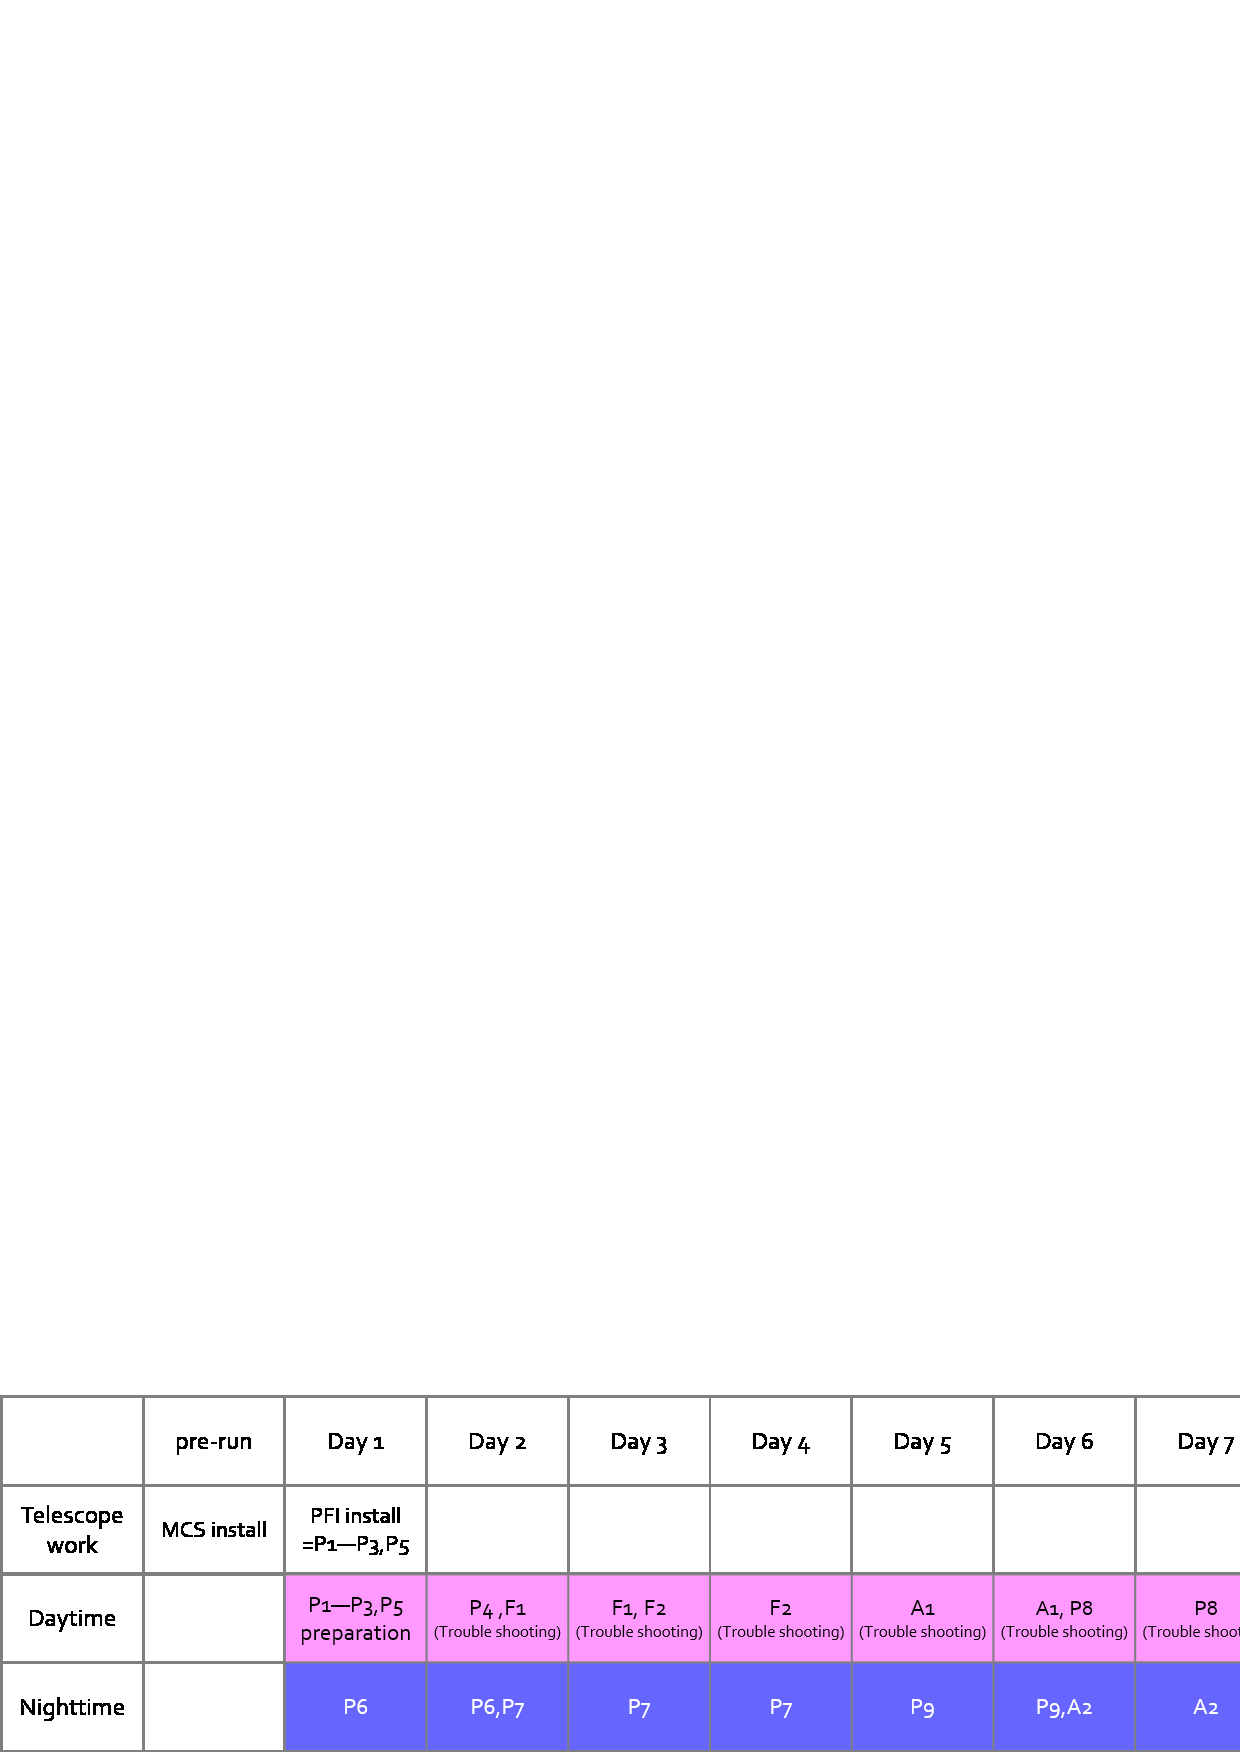
\includegraphics[width=108mm]{timetable_run2.pdf}
	\end{center}
	\vspace*{-5mm}
	\caption{Time table of Run 2.}
	\label{fig:run2}
\end{minipage}
\end{tabular}
\end{center}
\end{figure}

%---------------------------------------------------
% Run 3
%---------------------------------------------------
\begin{figure}[!ht]
\begin{center}
\begin{tabular}{c}
\begin{minipage}{0.95\hsize}
\paragraph{Run 3 : 10 days  (Figure \ref{fig:run3})}
During the telescope down-time for Mitsubish's test using PFS, we will use the nights to test Cobra using MCS. 
	\begin{itemize}
	\item 1 day (daytime) for P-1 -- P-3,  and F-1:
	(1) check PFI/POpt2 standing by,
	(2) install POpt2 to the prime focus,
	(3) check PFI functions, and
	(4) connect Cable B to PFI and SpS (SM1)
	\item 0.5 day (nighttime) for P-4 :
	(1) verify  MCS performance at zenith
	\item $\sim 5$ days (nighttime) for A-1 :
	(1) calibration of Cobras (all)
	\item $\sim 2$ days (1.0-day nighttime) for A-2 : 
	(1) PSF measurement through the entire system (SM1)	
	\item 1 day (nighttime) for P-4 and P-5 (after telescope can be moved):
	(1) measure x/y offset of PFI rotation center on MCS, and
	(2) verify  MCS performance at different elevation angle
	\end{itemize}
We also plan to take arc and flat images.
\end{minipage} \\
\begin{minipage}{0.8\hsize}
	\begin{center}
	\vspace*{5mm}
	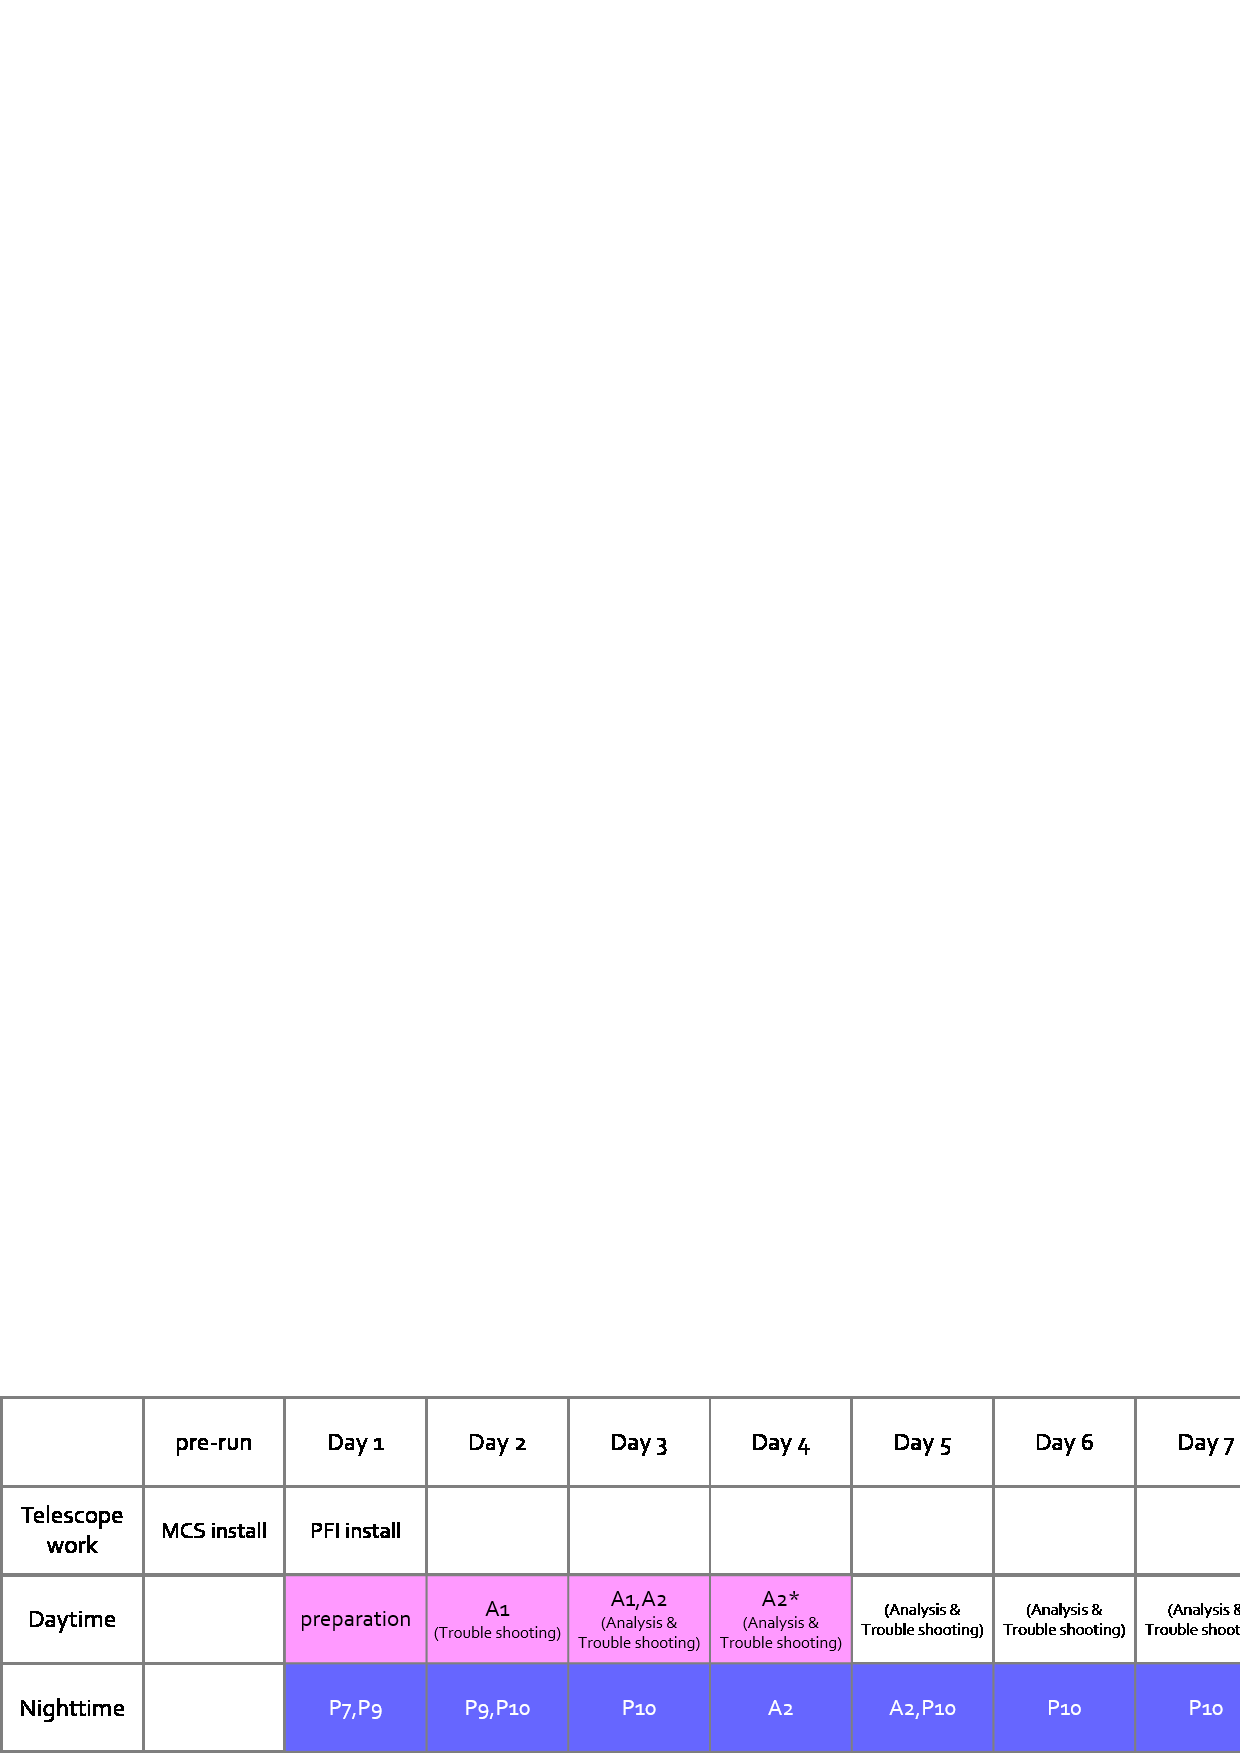
\includegraphics[width=120mm]{timetable_run3.pdf}
	\end{center}
	\vspace*{-5mm}
	\caption{Time table of Run 3.}
	\label{fig:run3}
\end{minipage}
\end{tabular}
\end{center}
\end{figure}


%---------------------------------------------------
% Run 4
%---------------------------------------------------
\begin{figure}[!ht]
\begin{center}
\begin{tabular}{c}
\begin{minipage}{0.95\hsize}
\paragraph{Run 4 : 7 days  (Figure \ref{fig:run4})}
	\begin{itemize}
	\item 1.2 $+$ 1.5 days (nighttime) for P-6 :
	(1) verification of A\&G camera functions (1.5 days is done with Mitsubishi)
	\item 1.0 days (nighttime) for P-7 :
	(1) correct WFC shift/tilt with respect to the primary mirror
	\item 1.5 days (daytime) for P-8 :  
	(1) confirm fixed fiducial fiber positions on F3C (refine the PFI-MCS relation)
	\item 1,5 days (nighttime) for P-9 :
	(1) Telescope Pointing Analysis (w/ith Mitsubishi)
%	\item 0.7 day (daytime) for F-1 : 
%	(1) connect Cable B to PFI and SpS (SM1/2/3)
	\item 0.5 days (daytime and/or nighttime) for A-1 : 
	(1) Test fiber allocation
	\item 1.0 days (1.0-day nighttime) for A-2 : 
	(1) PSF measurement through the entire system (SM1,2,3)	
\end{itemize}
The run 4 has 3-night work by/with Mitsubishi for test of software of the telescope control.
Note that we assume that we can coordinate with Mitsubishi to proceed some test items in parallel.
Note also that some test items such as AG functionality test and TPA will be done with Mitsubishi. 
The below is test items when we apply the engineering time in the S21B semester:
\begin{verbatim}
[a] POpt2 alignment, measure InR center using AG camera. [1 night]
[b] AG camera test and characterization [1.2 nights]
    - AG camera centroiding test (0.3 nights)
    - AG camera Orientation and pixel scale measurement (0.3 night)
    - Check focus position of AG focal plane and focusing test (0.4 night)
    - Field acquisition (0.2 night)
[c] Mitsubishi's test for AG [1.5 nights]
[d] Mitsubishi's test for PA [1.5 nights]
[e] Fiber allocation test [0.5 nights]
[f] PSF characterization for development of data reduction pipeline [1 night]
    - Sky spectra acquisition at different El and InR (0.5 nights x 2 sets). 
        (2 sets of images are needed to study time dependency)

    Note: In addition to night-time observation, the following tests need to be 
          done at the daytime. 
    - Measurement of PFI rotation center on MCS and check the repeatability 
      of installation. (0.1 day)
    - Check and refine the fixed fiducial fibers position on focal plane. (1 day)
    - Study effect of the Cobra position on PSF (0.5 day x 4 sets) 
\end{verbatim}
\end{minipage} \\
\begin{minipage}{0.8\hsize}
	\begin{center}
	\vspace*{5mm}
	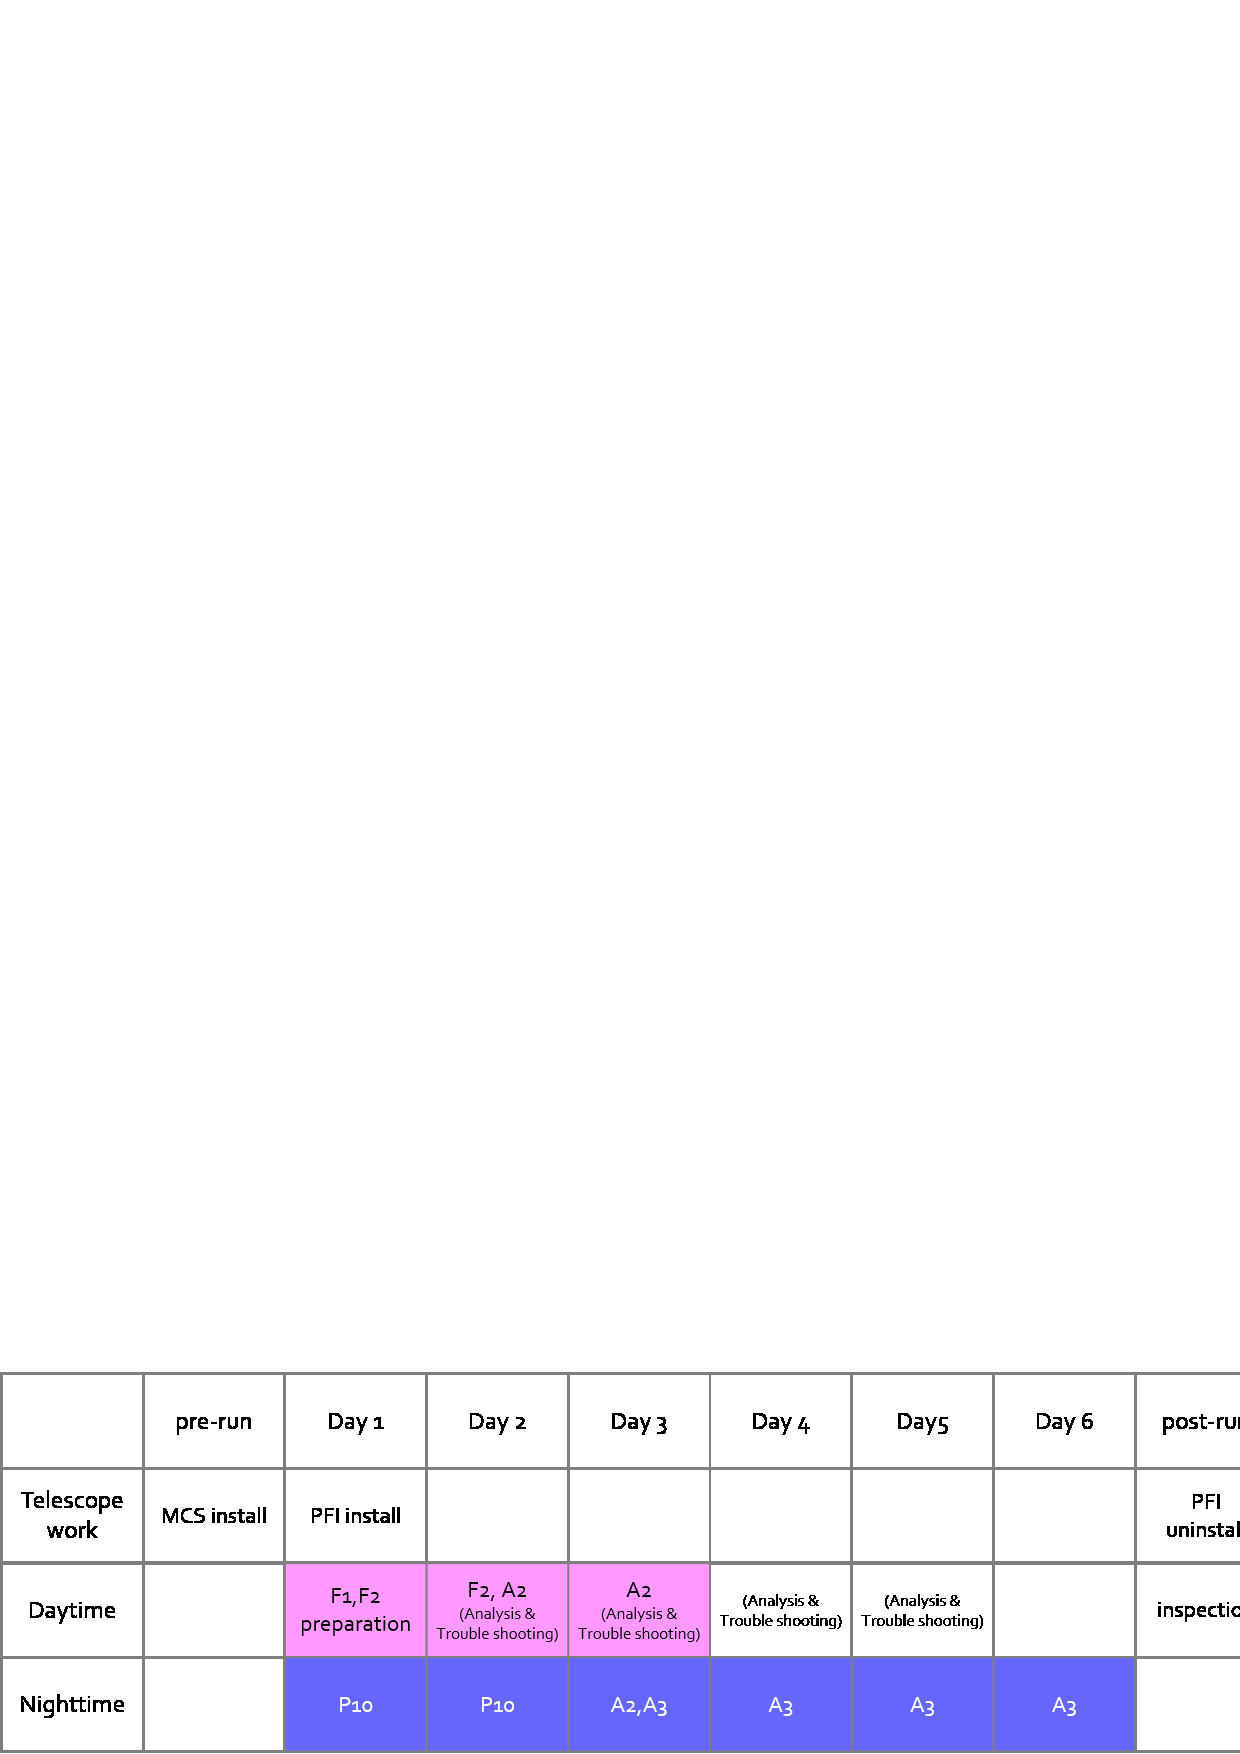
\includegraphics[width=120mm]{timetable_run4.pdf}
	\end{center}
	\vspace*{-5mm}
	\caption{Time table of Run 4.}
	\label{fig:run4}
\end{minipage}
\end{tabular}
\end{center}
\end{figure}

%---------------------------------------------------
% Run 5
%---------------------------------------------------
\begin{figure}[!ht]
\begin{center}
\begin{tabular}{c}
\begin{minipage}{0.95\hsize}
\paragraph{Run 5 : 5 days  (Figure \ref{fig:run5})}
	\begin{itemize}
	\item 0.2 days (nighttime) for P-6 :
	(1) check AG focus comparing with the focus of the science fibers.
	\item 0.3 days (nighttime) for P-7 :
	(1) correct WFC shift/tilt with respect to the primary mirror (confirmation)
	\item 0.1 days (nighttime) for P-9 :
	(1) Telescope Pointing Analysis (confirmation)
	\item 2 days (nighttime) for P-10 : 
	(1) 1st-pass distortion map
	\item 2.5 days (1.0-day daytime and 1-day nighttime) for A-2 : 
	(1) PSF measurement through the entire system (SM1)
	\item 1 day (nighttime) for A-3 : 
	(1)2nd-pass distortion map
	\end{itemize}
%If needed, we will connect SM1 to the Cable B for other Spectrograph Modules to see spatial variation for test \ref{secflow:PSFchar}
The below is test items when we apply the engineering time in the S21B semester.
Since 5 nights are allocated whereas 7 nights were applied, 1 nights are reduced for A-10 and A-3, respectively:
\begin{verbatim}
[a] POpt2 alignment and InR center confirmation (repeatability) [0.3 nights]
[b] Confirm telescope pointing [0.1 nights]
[c] Determine the AG camera coordinate system w.r.t. the fiducial fibers [1.5 nights] 
    - dithering around the AG fiducial fibers (2 fibers for each camera). 
    - El dependency confirmation
[d] Distortion study using astrometry data on AG camera [3 nights]
    - Study dependency of the instrument rotator
    - Study dependency on elevation
    - Study dependency on ADC position
      In total, ~50  set of data (1 set ~0.05 nights)
[e] Distortion study by taking star spectra (dithering around the allocated 
    position) [2 nights]
    - Do dithering (raster-scan) for ~20 fields at different El, N/S and InR and 
      refine fiber allocation. (0.1 nights per field)
[f] AG focus position measurement to compare with the science fibers focal plane 
    [0.2 nights]
[g] Take reference star spectra (radial velocity standard, telluric, abundance) for 
    data reduction pipeline [0.5 night]
[h] PSF characterization for development of data reduction pipeline [1 night]
    - Sky spectra acquisition at different El and InR  (0.5 nights x 2 sets)

    Note: In addition to night-time observation, the following tests need to be 
          done at the daytime. 
   - Study effect of the Cobra position on PSF (repeatability) (0.25 day x 4 sets) 
\end{verbatim}
\end{minipage} \\
\begin{minipage}{0.8\hsize}
	\begin{center}
	\vspace*{5mm}
	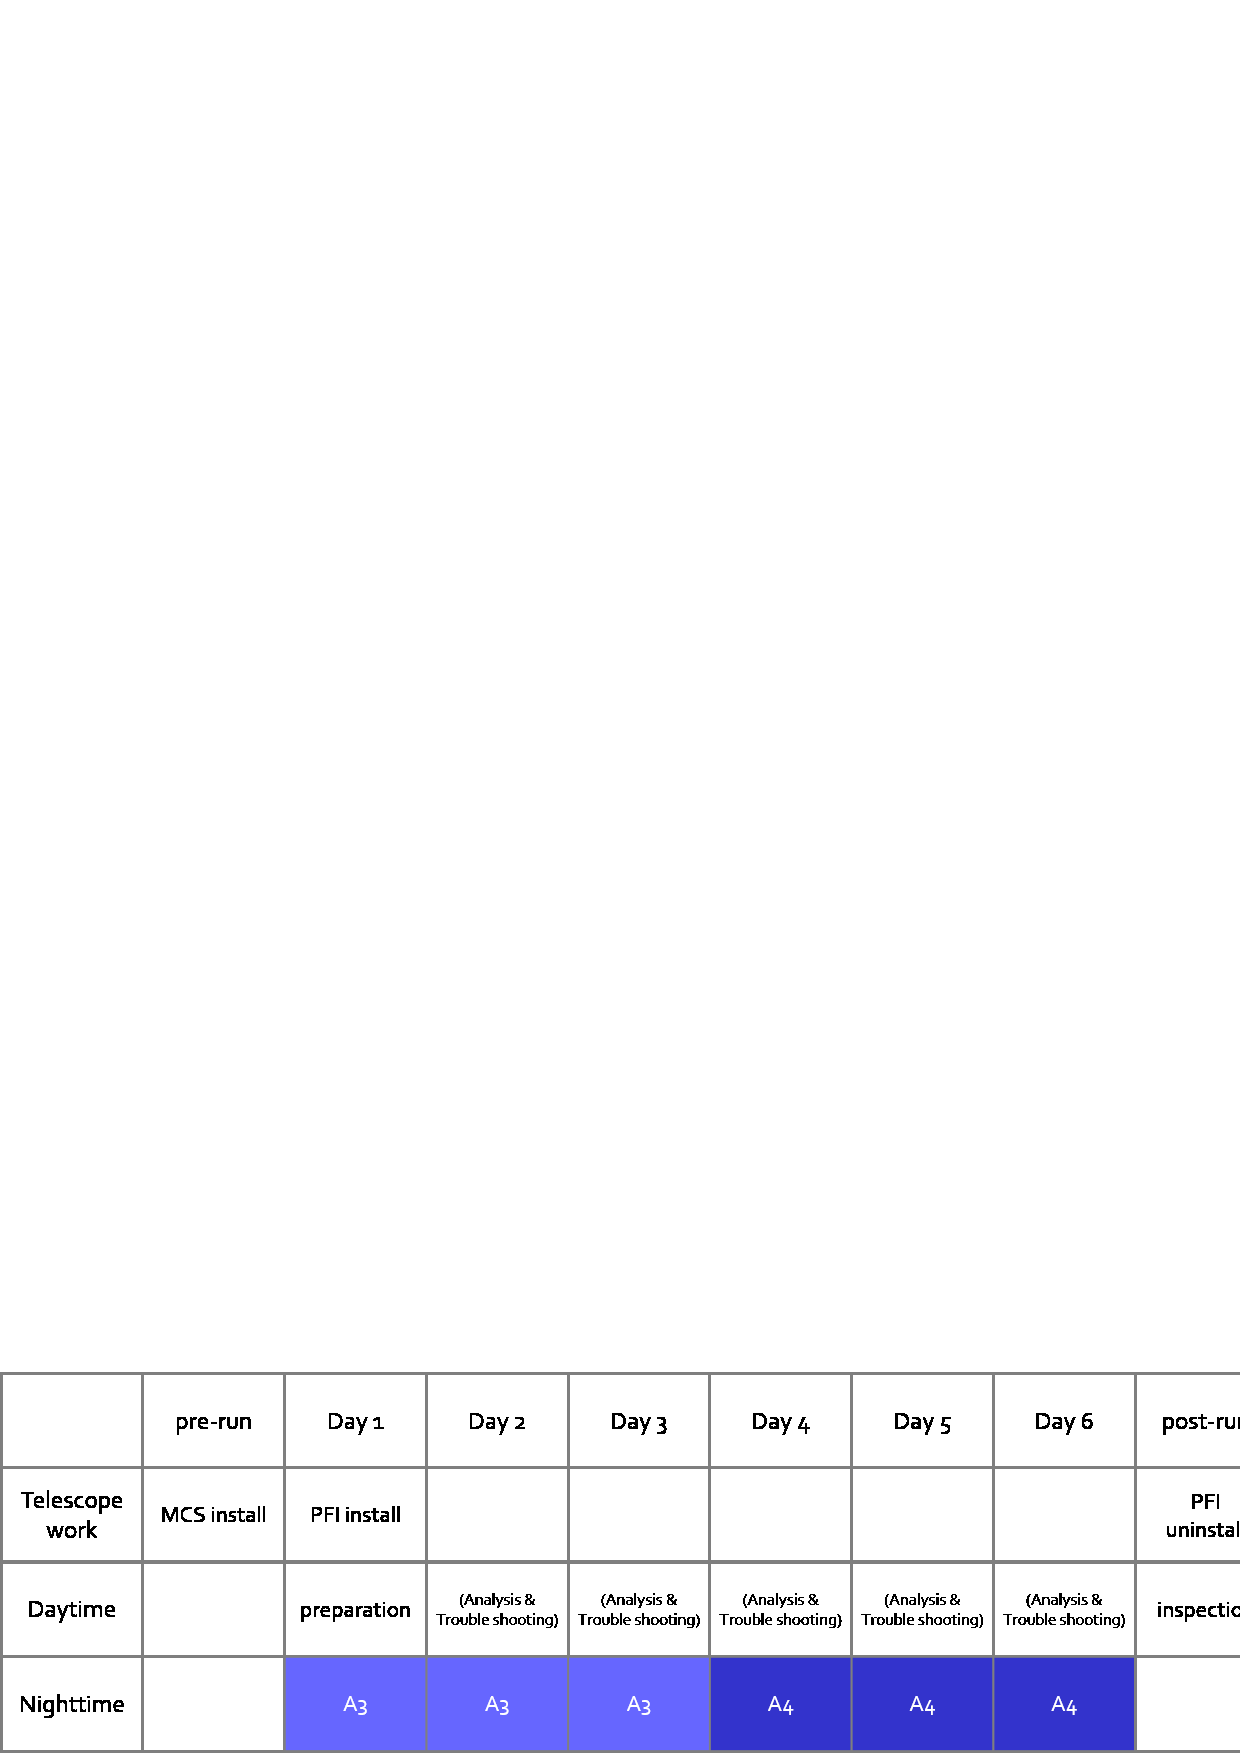
\includegraphics[width=98mm]{timetable_run5.pdf}
	\end{center}
	\vspace*{-5mm}
	\caption{Time table of Run 5.}
	\label{fig:run5}
\end{minipage}
\end{tabular}
\end{center}
\end{figure}

%---------------------------------------------------
% Run 6
%---------------------------------------------------
\begin{figure}[!ht]
\begin{center}
\begin{tabular}{c}
\begin{minipage}{0.95\hsize}
\paragraph{Run 6 : 6 days  (Figure \ref{fig:run6})}
	\begin{itemize}
	\item 2 days (nighttime) for P-10 : 
	(1) 1st-pass distortion map
	\item 0.5 day (daytime) for F-1 :  
	(1) connecting Cable B to PFI and SpS (SM2,3,4)
	\item 1.0 day (daytime) for F-2 :  
	(1) confirmation of  the fiber identifications (SM2,3,4)
	\item 1.5 days (1.0-day daytime and 0.5-day nighttime) for A-2: 
	(1) PSF measurement through the entire system (all but SM4-NIR)
	\item 3.5 days (nighttime) for A-3: 
	(1) 2nd-pass distortion map
	\end{itemize}
% If needed, we will connect SM1 to the Cable B for other Spectrograph Modules to see spatial variation for test \ref{secflow:raster}
\end{minipage} \\
\begin{minipage}{0.8\hsize}
	\begin{center}
	\vspace*{5mm}
	\includegraphics[width=108mm]{timetable_run6.pdf}
	\end{center}
	\vspace*{-5mm}
	\caption{Time table of Run 6.}
	\label{fig:run6}
\end{minipage}
\end{tabular}
\end{center}
\end{figure}


%---------------------------------------------------
% Run 7
%---------------------------------------------------
\begin{figure}[!ht]
\begin{center}
\begin{tabular}{c}
\begin{minipage}{0.95\hsize}
\paragraph{Run 7 : 6 days  (Figure \ref{fig:run7})}
	\begin{itemize}
	\item 4 days (nighttime) for A-3: 
	(1) 2nd-pass distortion map
	\item 2 days (dark-night) for A-4 :
	(1) performance verification I (all but SM4-NIR)
	\end{itemize}
\end{minipage} \\
\begin{minipage}{0.8\hsize}
	\begin{center}
	\vspace*{5mm}
	\includegraphics[width=108mm]{timetable_run7.pdf}
	\end{center}
	\vspace*{-5mm}
	\caption{Time table of Run 7.}
	\label{fig:run7}
\end{minipage}
\end{tabular}
\end{center}
\end{figure}

%---------------------------------------------------
% Run 8
%---------------------------------------------------
\begin{figure}[!ht]
\begin{center}
\begin{tabular}{c}
\begin{minipage}{0.95\hsize}
\paragraph{Run 8 : 5 days  (Figure \ref{fig:run8})}
	\begin{itemize}
	\item 2.0 days (1.0-day daytime and 1.0-day nighttime) for A-2: 
	(1) PSF measurement through the entire system (all SMs)
	\item 4 days (dark-night) for A-4 and A-5 : 
	(1) performance verification I (SM1/2/3),  and
	(2) performance verification II (stabilization, using SM1/2/3)
	\end{itemize}
\end{minipage} \\
\begin{minipage}{0.8\hsize}
	\begin{center}
	\vspace*{5mm}
	\includegraphics[width=98mm]{timetable_run8.pdf}
	\end{center}
	\vspace*{-5mm}
	\caption{Time table of Run 8.}
	\label{fig:run8}
\end{minipage}
\end{tabular}
\end{center}
\end{figure}

%---------------------------------------------------
% Run 9 and 10
%---------------------------------------------------
\begin{figure}[!ht]
\begin{center}
\begin{tabular}{c}
\begin{minipage}{0.95\hsize}
\paragraph{Runs 9 and 10 : 4 days  (Figure \ref{fig:run9})}
	\begin{itemize}
	\item 4 days (dark-night) for A-5 :
	(1) performance verification II (stabilization)
	\end{itemize}
\end{minipage} \\
\begin{minipage}{0.8\hsize}
	\begin{center}
	\vspace*{5mm}
	\includegraphics[width=84mm]{timetable_run9.pdf}
	\end{center}
	\vspace*{-5mm}
	\caption{Time table of Runs 9 and 10.}
	\label{fig:run9}
\end{minipage}
\end{tabular}
\end{center}
\end{figure}


%--------------------------------------------------------------
%  Table: expected runs and nights
%--------------------------------------------------------------
\setlength{\tabcolsep}{1mm}{
\begin{table}[!ht]
\begin{center}
\caption{
Expected number of working days for commissioning (as of June 2021).
Column 1 lists the run number.
Year/Month in column 2 are just roughly set  for the Run 6 and later assuming the latest schedule of each subsystems and that scientific operation will start in the S23B  semester.
The required days for each run are listed in column 3.
Required days for individual  processes at each run are listed in column 5 (daytime) or 6 (night-time).
The numbers in parentheses in column 6 is required dark nights.  
}
%\scriptsize
\footnotesize
\begin{tabular}{*{3}{c}|*{3}{c}}\label{tbl:CountDates} \\ \hline
Run	 & Year/Month  &\#days & process	& daytime & night (dark) \\ \hline \hline
0	& S17B--S21A			& 4.5***	& P7(*) etc.	& 0		& 7.0 (2.5)	\\ \hline
--	& 2018/06			& --		& M1		& --		& --	\\ \hline
1	& 2018/10			& 3		& M1--3		& (1**)	& 0	(0)	\\
	& 	& 				& M4, ASIAA	& 0		& 3	(0)	\\ \hline
2	& 2019/08	& 5				& M4, M3, ASIAA	& 0		& 5	(0)	\\ \hline
--	& 2019/12--2020/01			& --		& S1,S2 (SM1:B+R)		& --		& --	\\ \hline
3	& 2021/09	& 10****			& P1--P3,F1 (SM1)	& 	& 0.5 (0)	\\
	&	&					& P4,P5			& 0 	& 1.5 (0)	\\
	&	&					& A1	& 0 	& 5.0 (0)	\\
	&	&					& A2 (SM1B+R)	& 0 	& 2.0 (0)	\\ \hline
4	& 2021/10	& 7***			& P6  			& 0 	& 2.7*** (0)	\\
	&	&					& P7  			& 0 	& 1.0 (0)	\\
	&	&					& P8  			& 1.5 	& 0 (0)	\\
	&	&					& P9  			& 0 	& 1.5*** (0)	\\
	&	&					& A1	& 0.5 	& 0 (0)	\\
	&	&					& A2 (SM1,2,3)	& 0 	& 1.0 (0)	\\ \hline
5	& 2021/11	& 5 		& P6 			& 0 	& 0.2 (0)	\\
	&	&					& P7 			& 0 	& 0.3 (0)	\\
	&	&					& P9  			& 0 	& 0.1 (0)	\\
	&	&					& P10  			& 0 	& 2 (0)	\\
	&	&					& A2 (SM1)	& 1 	& 1 (0)	\\ 
	&	&					& A3 			& 0 	& 1 (0)	\\ \hline
--	& 2022/early			& --		& S1,S2 (SM2:B+R)		& --		& --	\\ 
--	& 2022/early			& --		& S1,S2 (SM3)		& --		& --	\\ 
--	& 2022/early			& --		& S1,S2 (SM4:B+R)		& --		& --	\\
--	& 2022/middle			& --		& S1,S2 (SM1:N)		& --		& --	\\ \hline
6	& 2022/05	& 6 		& P10 			& 0 	& 2 (0)	\\
	&	&					& A2 (SM1,2,3)	& 1 	& 0.5 (0)	\\
	&	&					& A3 			& 0 	& 3.5 (0)	\\ \hline
--	& 2022/middle			& --		& S1,S2 (SM2:N)		& --		& --	\\ \hline
7	& 2022/07	& 6					& A3			& 0		& 4 (0)	\\
	&	&					& A4			& 0		& 0 (2)	\\ \hline
--	& 2022/07			& --		& S1,S2 (SM4:N)		& --		& --	\\ \hline
--	& 2022/middle			& --		& S1,S2 (SM4:N)		& --		& --	\\ \hline
8	& 2022/10	& 5			& A2 (all SMs)	& 1 	& 1 (0)	\\
	&	&					& A4			& 0		& 0	(2)	\\
	&	&					& A5			& 0		& 0 (2)	\\ \hline
9	& 2022/12	& 4			& A5			& 0		& 0 (4)	\\ \hline
19	& 2023/02	& 4			& A5			& 0		& 0 (4)	\\ \hline \hline
\multicolumn{2}{r}{in total}& 45 (52***) \\ \hline
\end{tabular}
\\
* Check algorithm at HSC engineering run. \\
** Telescope can be used for other instruments \\
*** The number combined with run 0 and Mitsubishi's work \\
**** During telescope downtime for Mitsubishi's test (the number of used night is not counted)
\end{center}
\end{table}

\clearpage

\subsection{Relationship among Individual Sequence}
Some processes can be carried out in parallel, but some should in series.
Table \ref{tbl:Rel_Seq} shows the relationship among the individual sequences.
Each row displays commissioning processes related to each process in the columns.
``X" means required process.
For example, prior to the process M--3, M--2 (and hence M--1) should be succeeded.

%--------------------------------------------------------------
%  Table: the relation ship of commissioning sequence 
%  A sequence (top) marked with X is need prior to other sequence (row)
%--------------------------------------------------------------
\begin{table}[!ht]
\caption{
The relation of commissioning processes.}
\label{tbl:Rel_Seq}
\begin{center}
\includegraphics[width=170mm]{relationship_sequences.eps}
\end{center}
\end{table}


